\documentclass{beamer}
\usepackage[utf8]{inputenc}
\usepackage[]{hyperref}

\usepackage{booktabs,tabularx}
\usepackage{multicol,wrapfig,setspace}

\usetheme[pageofpages=of,bullet=square,
	titleline=true,
	alternativetitlepage=true,
	titlepagelogo=figs-slides/icon-dta.jpg]{Torino}

\author{Statistical Reasoning\\and Quantitative Methods}
\title{Datasets}
\institute{François Briatte \& Ivaylo Petev}
\date{Session 2}

\include{beameradditions}

\begin{document}
		
	\begin{frame}[t,plain]
		\titlepage
	\end{frame}
	
	\begin{frame}[t]{Outline}
	
	Quantitative data come as \red{datasets} in particular formats. Your research projects will use \red{cross-sectional data} in Stata format (\code{.dta}).
	
		\begin{columns}[T]
		\column{.35\textwidth}
			\tableofcontents[hideallsubsections]
		\column{.6\textwidth}
			\begin{center}
				
\includegraphics[scale=.25]{figs-slides/icon-dta.jpg}
			\end{center}		
		\end{columns}
	\end{frame}
	

	%
	%
	%	
	\section{Objectives}
	%
	%
	%

	\begin{frame}[t]{Objectives}

	At the early stage of your project, you will look for \red{cross-sectional data}, which is a \red{time-consuming task}. Consider yourself done only when the dataset is open and ready for analysis in Stata.\vspace{1em}

		\begin{itemize}
			\item \textbf{Find a dataset,} based on availability and research interests.
			
			\item \textbf{Download its documentation,} and especially the codebook. 
			
			\item \textbf{Convert and reshape} if necessary (Stata Guide, Section 7).
			
			\item \textbf{Explore and describe} by writing up a draft do-file.
		\end{itemize}\vspace{1em}
	
	It is strongly recommended that you have formed pairs and have a Stata dataset ready for exploration \red{by next week.} The results of your exploratory analysis will later appear in Assignment No.~1.
	
	\end{frame}

	\section{Structure}

	\subsection{Data structure}
	
	\begin{frame}[t]{Data structure}

	\textbf{Cross-sectional data} capture the characteristics of a \red{sample} of comparable \red{units} at a \red{single point} in time:

	\begin{itemize}
		\item \textbf{Units} can be individual respondents, states, organizations…
		\item \textbf{Observations} vary by their characteristics, \textit{not} by unit type
		\item \textbf{Sampling} will vary depending on representativity requirements
	\end{itemize}
		
	\textbf{Time series} capture \red{repeated} observations over time of either sampled or nonsampled units:

	\begin{itemize}
		\item \textbf{Cross-sectional time series} (CSTS) capture fixed, nonsampled units at different time intervals
		\item \textbf{Longitudinal data} capture sampled units (called cohort or panel) at different time intervals
	\end{itemize}

	\end{frame}
	
	\subsubsection{Example}
	
	\begin{frame}[t]{\textit{Example:} \href{http://www.ic.gc.ca/eic/site/ic1.nsf/eng/01464.html}{Industry Canada File Sharing Survey (2006)}}

	Using individual-level `micro' data on illegal downloading practices among a representative sample of the Canadian population aged 15+:\\[1em]
	
	\includegraphics[width=\textwidth]{figs-slides/cross-sectional.png}

	\begin{itemize}
		\item \textbf{Observations:} rows hold data for a single sampled unit
		\item \textbf{Variables:} columns hold all values for a single variable
		\item \textbf{Missing data:} ``Do Not Know / Refused to Answer'', `\code{.}'
		\item \textbf{Value formats:} numeric, \rd{string}, \bl{encoded} (values/labels)
	\end{itemize}
	
	\end{frame}

	\subsection{Format requirements}
	
	\begin{frame}[t]{Format requirements}
	
	Check your dataset against the following list:

		\begin{itemize}
			\item The dataset format is \textbf{DTA} (\code{.dta}).\\
			\textit{Otherwise, non-Stata format: \red{convert}.}
			
			\item The data are available at \textbf{only one point in time} (e.g. year 2009).\\
			\textit{Otherwise, time series: \red{subset}.}
		
			\item The columns do \textbf{not hold time variables} (e.g. y1960, y1961, …)\\
			\textit{Otherwise, `wide' data: \red{reshape}.}
		\end{itemize}
			
	If you need to reformat your dataset before analysing it, all guidelines and operations are detailed in the Stata Guide, Sections 5--8.
	
	\end{frame}

	%
	% AVAILABILITY
	%
	
	\section{Availability}

	\begin{frame}[t]{Availability}
	
	Generally speaking, things are getting much better:

		\begin{itemize}
		\item \textbf{``Data Deluge'':} scientists, journalists and organizations share more and more data online.

		\item \textbf{Open formats:} converting, expanding and sharing data through different media is increasingly possible.
		
		\item \textbf{Visualization projects:} online platforms that support graphical views of data are becoming very popular.
				
		\end{itemize}
	
		For a few examples, check the \textit{Guardian}'s Data Blog:
		
		\url{http://www.guardian.co.uk/news/datablog}\\[1em]
		
		More relevant links appear in the \texttt{README} file of the \texttt{Datasets} folder, as well as on the course blog:
				
		\url{http://srqm.tumblr.com/tagged/data}
	
	\end{frame}
	
	\begin{frame}[t]{\textit{Example:} \href{http://www.gapminder.org/}{Gapminder}}

	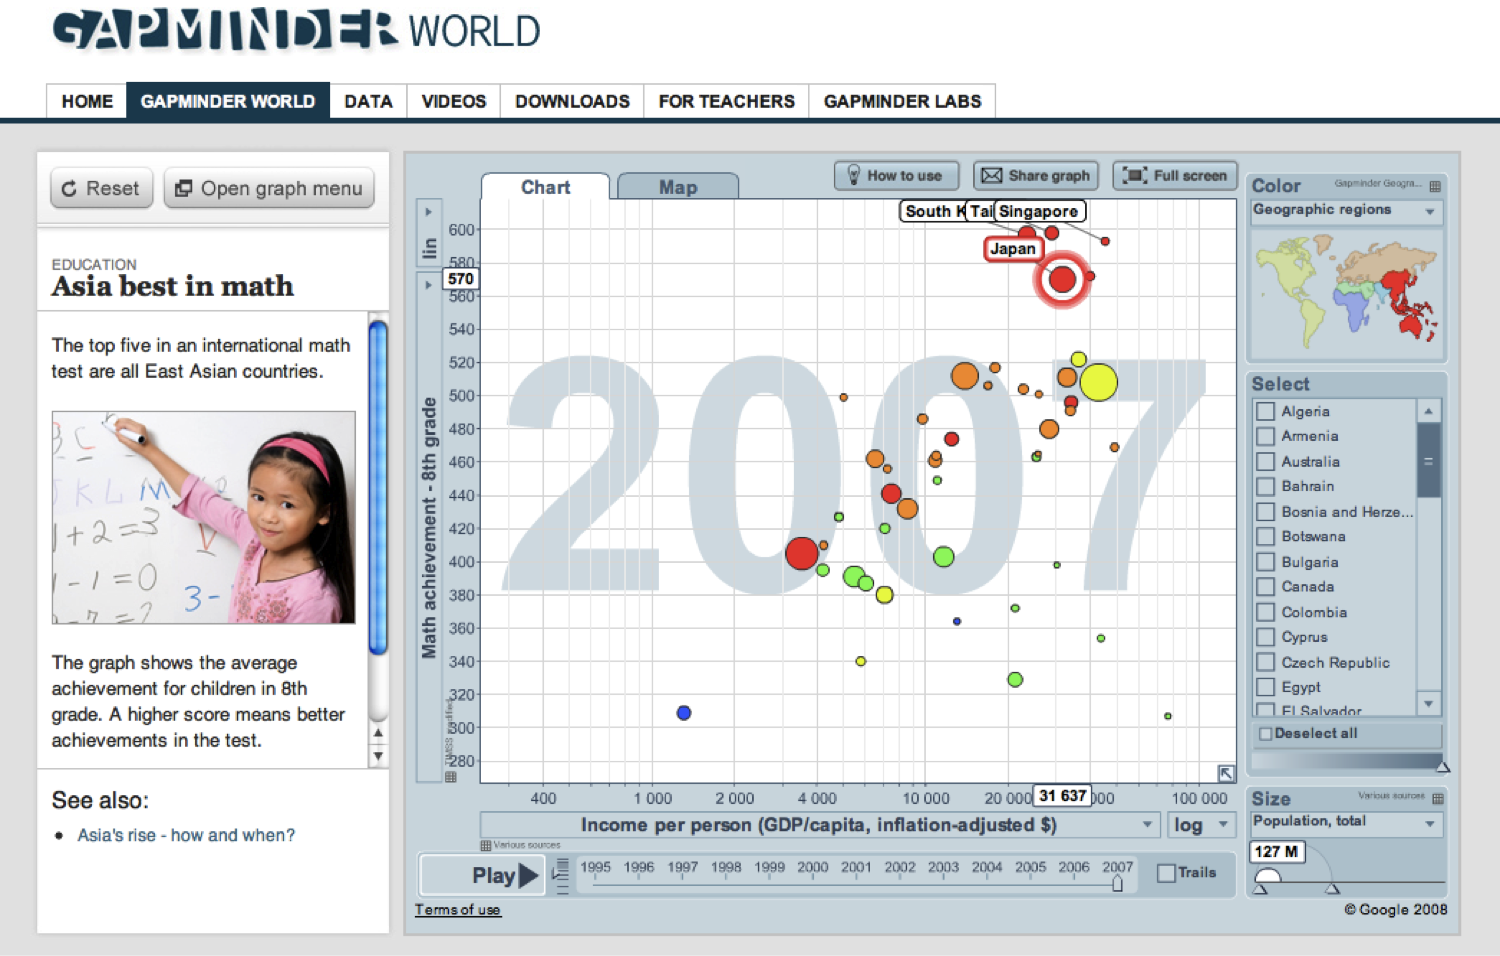
\includegraphics[width=\textwidth]{figs-slides/gapminder.png}

	\end{frame}
	
	\subsection{Recommended sources}

	\begin{frame}[t]{Recommended sources}
	
	Start with recommended datasets and repositories:

		\begin{itemize}
		\item \textbf{Teaching Pack $\triangleright$ Datasets}:

				\begin{itemize}
				\item \textbf{ESS 2008}: European Social Survey

				\item \textbf{WVS 2000}: World Values Survey

				\item \textbf{QOG 2011}: Quality of Government
			\end{itemize}
			
			\red{Note:} consult with us if you are planning to use a dataset that is not from the Teaching Pack.

			\item \textbf{\texttt{Datasets/README} $\triangleright$ Datasets}:
		
			\begin{itemize}
				\item \textbf{ICPSR}: \url{http://www.icpsr.umich.edu/}
		
				\item \textbf{CESSDA}: \url{http://www.cessda.org/}
		
%				\item \textbf{IPSAportal}: \url{http://ipsaportal.unina.it/?cat=16}				
			\end{itemize}
					
			\red{Note:} some data sources will ask you to register online before granting you full access.
				
		\end{itemize}
	
	\end{frame}

	\subsubsection{Examples}
	
	\begin{frame}[t]{\textit{Example:} \href{http://www.icpsr.umich.edu/}{ICPSR} (topic search: Health)}

	\includegraphics[width=\textwidth]{figs-slides/data-icpsr1.png}

	\end{frame}

	\begin{frame}[t]{\textit{Example:} \href{http://www.icpsr.umich.edu/}{ICPSR} (variable search: Presidential)}

	\includegraphics[width=\textwidth]{figs-slides/data-icpsr2.png}

	\end{frame}
	
	\begin{frame}[t]{\textit{Example:} \href{http://www.icpsr.umich.edu/}{ICPSR} (geography search: Russia)}

	\includegraphics[width=\textwidth]{figs-slides/data-icpsr3.png}

	\end{frame}

	\begin{frame}[t]{\textit{Example:} \href{http://www.cessda.org/}{CESSDA} (keyword search: Legal Systems)}

	
\includegraphics[width=\textwidth]{figs-slides/data-cessda.png}

	\end{frame}
		


	\subsection{Source requirements}

	\begin{frame}[t]{Source requirements}
	
	You need to be able to reference your dataset in full before use. This implies collecting information on:

		\begin{itemize}
			\item \textbf{the source}, with its full name and online address\\
			\textit{e.g. World Health Organization (WHO), [website]}
			
			\item \textbf{the unit of analysis}, with its restrictions\\
			\textit{e.g. American adult resident population with U.S. citizenship}
			
			\item \textbf{the sampling strategy}, with a reference if needed\\
			\textit{e.g. ``cf. `Sample Design' in the Survey Description [source]''}
			
			\item \textbf{the total number of observations}\\
			\textit{e.g.} $N=1,524$
		\end{itemize}
			
	\red{Note:} all these characteristics need to appear in your research project.
	
	\end{frame}
	
	%
	%
	%
	\section{Exploration}
	%
	%
	%
	
	\subsection{Documentation}

	\begin{frame}[t]{Exploring the \red{documentation}}
		
	\textbf{Knowing the data is not an option.} You naturally do not have to `read' through the data itself, but \red{you need to read everything else}.\\[1em]
	
	The \textbf{codebook} is essential to \red{measurement}:		
		\begin{itemize}
			\item Data collection and measurement are publicly documented to allow for sceptical scrutiny of sources and method.
			\item The unit of continuous data, scale of ordinal data or categories of nominal data are given with their construction notes.
		\end{itemize}
	
	\end{frame}
	
	\subsection{Example}
	
	\begin{frame}[t]{\textit{Example:} Measurement}
		\begin{center}
			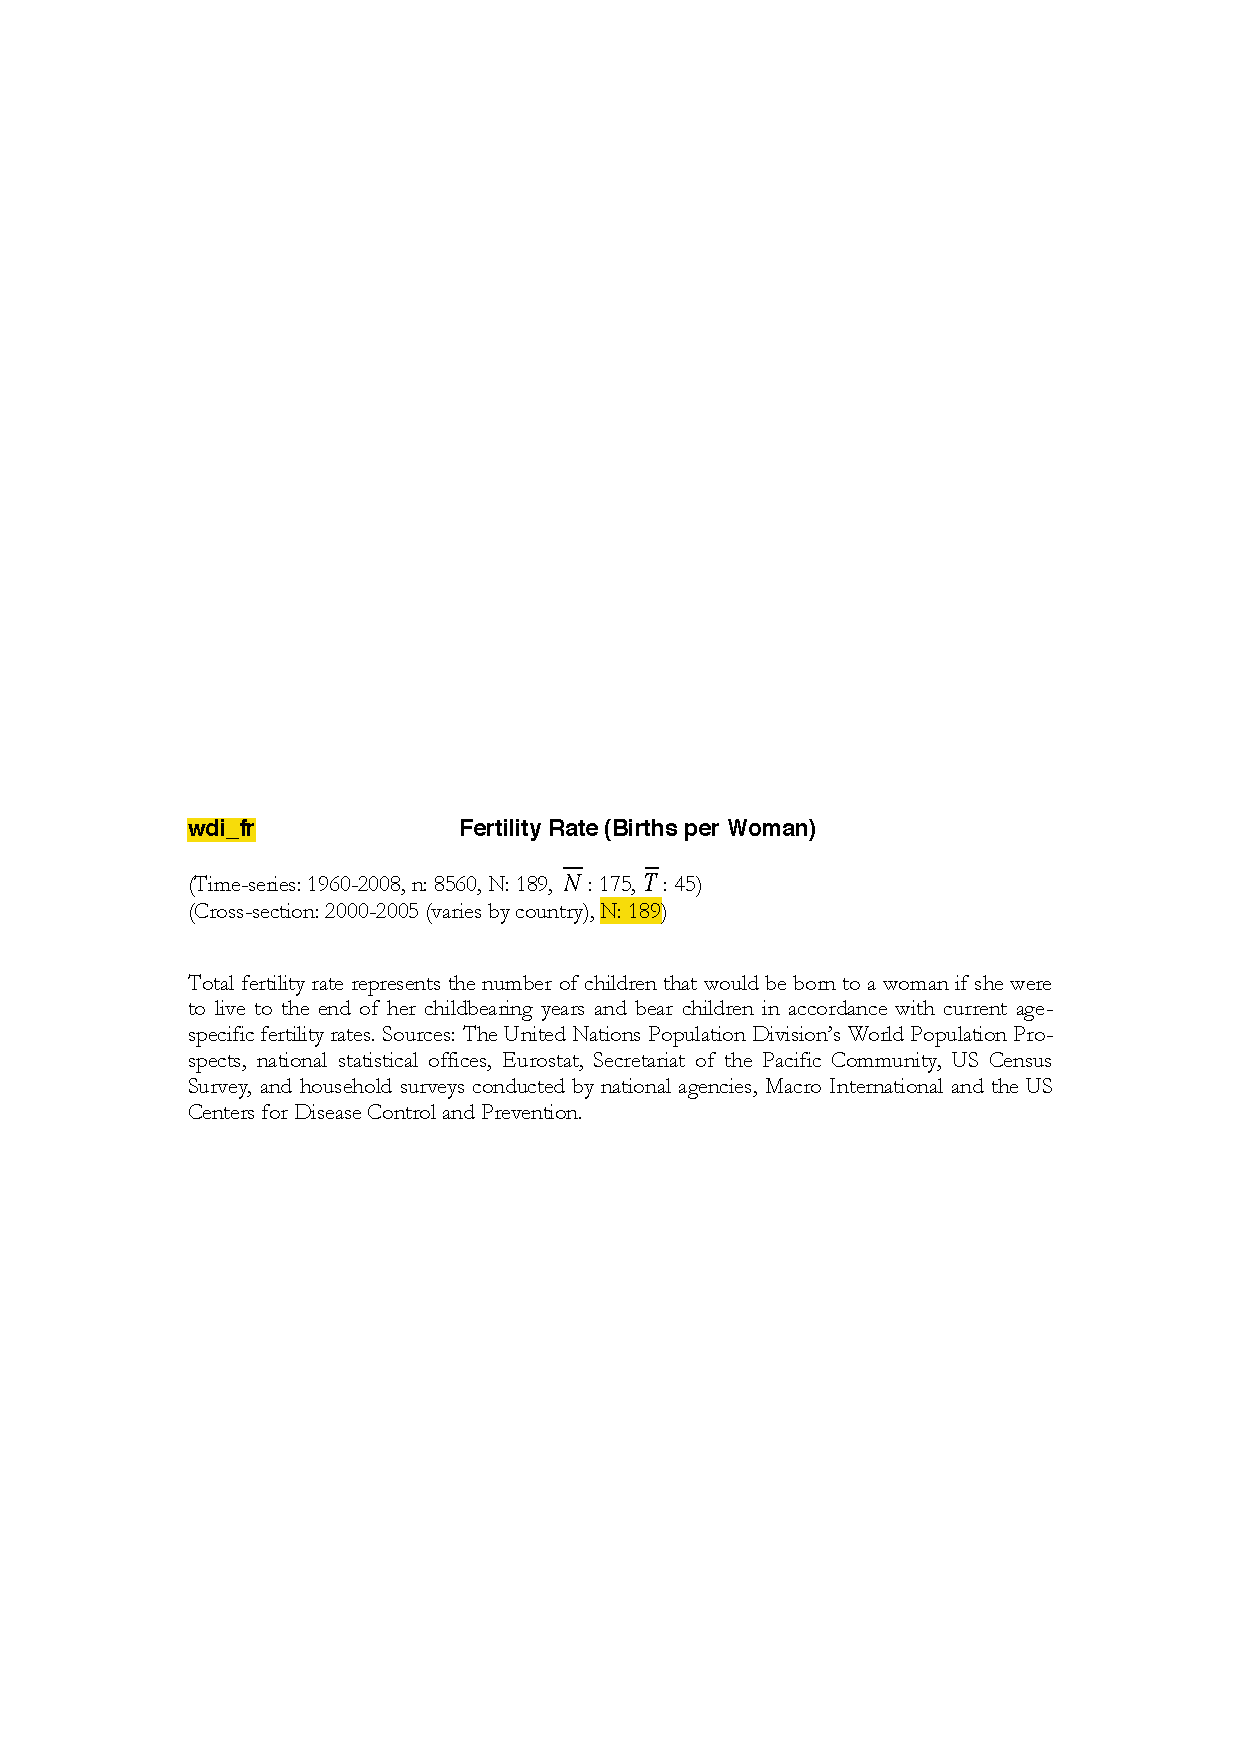
\includegraphics[width=\textwidth]{figs-slides/codebook-qog.jpg}		
		\end{center}
		%In the cross-sectional version of the dataset, the variable \code{wdi\_fr} was measured from 1999 to 2002 in $N=186$ units (countries).
	\end{frame}

	%
	
	\subsection{Identifiers}

	\begin{frame}[t]{Exploring the \red{identifiers}}
		
	\textbf{Data comes with identifiers:} \red{variables} have names and labels, and their values can also carry a label.\\[1em]
	
	Identifiers are essential to \red{writing commands}:
	
		\begin{itemize}
			\item Passing commands requires correct variable names, labels and values, as in \code{su rlgdgr if rlgdnm==6}.
			
			\item Excluding missing values frequently requires recoding them to the Stata \code{.} symbol(s) and passing the \code{if !mi()} selector.
		\end{itemize}
	
	\end{frame}

	\subsubsection{Example}
	
	\begin{frame}[t]{\textit{Example:} Coding}
		\begin{center}
			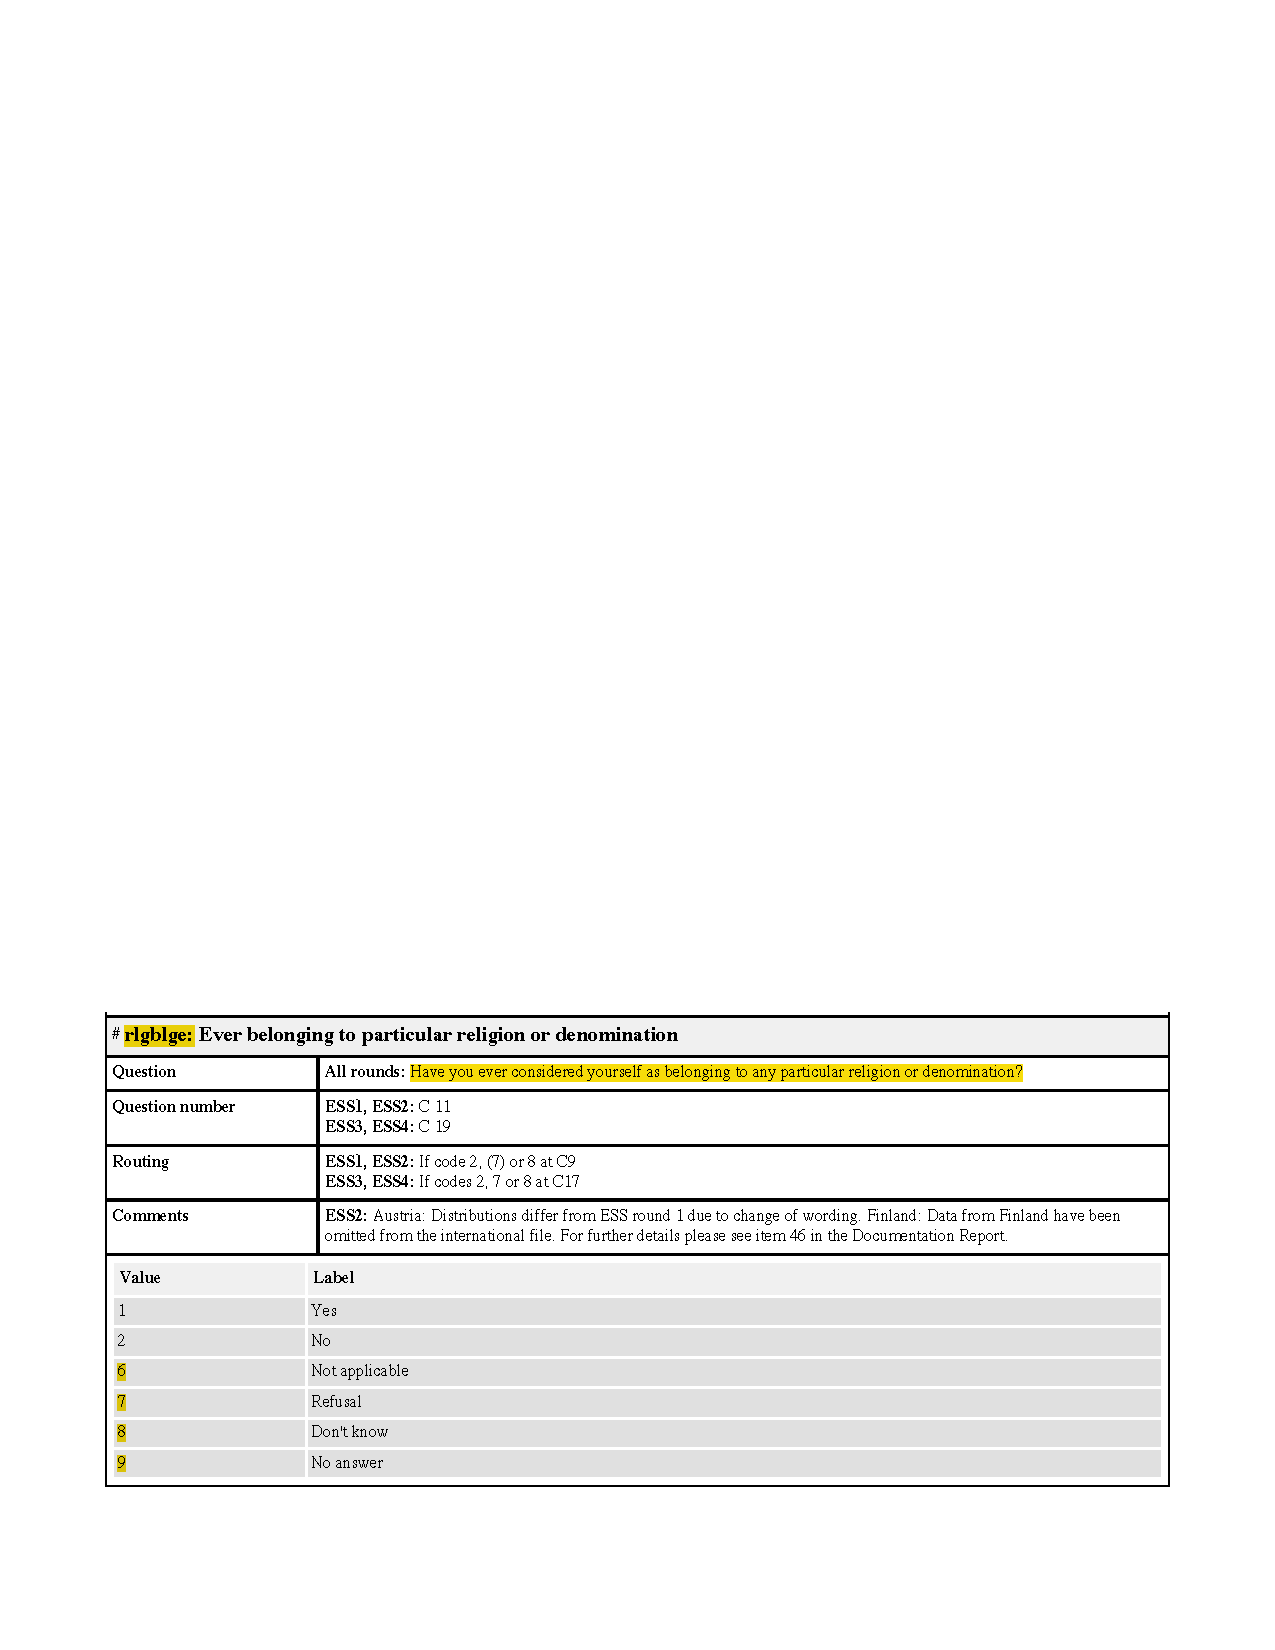
\includegraphics[width=\textwidth]{figs-slides/codebook-ess.jpg}		
		\end{center}
		%The variable named \code{dscrgrp}, labelled as ``Member of a group discriminated…'', takes 5 unique values, three of which code for missing values.
	\end{frame}
		
	%

	\subsection{Selections}
	
	\begin{frame}[t]{Selections}
	
	Stata offers two ways to select observations:

	\begin{itemize}
		\item \textbf{Range selection} with \code{in}:
		
		\begin{itemize}
		
			\item All observations have a row number \code{\_n} between 1 and sample size \code{\_N}. The number is arbitrary and non statistically meaningful.
	
			\item Range selection is principally useful to look at a few observations.

			e.g. \code{list in 1/10}, \code{list in -25/l}
		
		\end{itemize}
				
		\item \textbf{Logical selection} with \code{if}:
		
			\begin{itemize}
				\item ``equal to'' (\code{==}) or ``not equal to'' (\code{!=})
				\item ``greater/lesser than'' (\code{\textgreater/\textless}) and ''… or equal to''  (\code{\textgreater=/\textless=})
				
				\item ``and'' (\code{\&}), ``or'' (\code{|})
				\item ``missing'' (\code{mi()}) or ``nonmissing'' (\code{!mi()})
				
			\end{itemize}
			
			Logical operators apply to virtually all data operations.

	\end{itemize}
	
	\end{frame}

	\subsubsection{Examples}
	
	\begin{frame}[t]{Examples}
	
	Think of selecting observations as formulating linguistic statements:

	\begin{itemize}
		\item \textbf{Identification}, e.g. ``I am not Sidney Poitier''\\
		\code{drop if name=="Sidney Poitier"}
		
		\item \textbf{Validity}, e.g. ``Raise your hand if you're absent''\\
		\code{gen vote=1 if absent==1}
		
		\item \textbf{Conditions}, e.g. ``Twist and Shout''\\
		\code{replace beatles=1 if !mi(twist) \& !mi(shout)}
	\end{itemize}
	
	That logic allows to run commands on particular groups:
	
	\begin{itemize}
		\item \code{drop if mi(age) | age \textless~65} means\\``drop all observations where age is missing \textit{or} under 65.''
		\item \code{li country if gdp \textgreater= 5000 \& !mi(gdp)}'' means\\``list country if GDP is above or equal to 5,000 \textit{and} nonmissing.''
	\end{itemize}
	\end{frame}
	
	%
	%
	%
	\section{Practice}
	%	
	% (15 slides)
	%
		
	\subsection{Practice: Body Mass Index}
	
	\begin{frame}[t]{\textit{Practice:} \red{Body Mass Index}}

		$$\mathsf{BMI} = \frac{\mbox{mass} \ \mbox{(kg)}}{\left( \mbox{height}(\mathsf{m})\right)^2} = \frac{\mbox{mass} \ \mathsf{(lb)} \times 703}{\left(\mbox{height} (\mathsf{in})\right)^2}$$

		\begin{itemize}
			\item For \textbf{normal weight} adults, $18.5 < \mathsf{BMI} < 25$.

			\item For \textbf{overweight} adults, $25 \leq \mathsf{BMI} < 30$.
			
			\item For \textbf{obese }adults, $\mathsf{BMI} \geq 30$.
						
		\end{itemize}

		\begin{columns}[T]
			\column{.725\textwidth}
			
			\begin{itemize}
				\item National Health Interview Survey (NHIS)
				\item Sample: U.S. adult population, 1997--2009
			\end{itemize}

			\column{.2\textwidth}
			\includegraphics[scale=.6]{figs-slides/nhis.jpg}
		\end{columns}
		
	\end{frame}

	\subsection{Maps}
	
	\fullslide{figs-slides/cdc1.jpg}
	\fullslide{figs-slides/cdc2.jpg}
	\fullslide{figs-slides/cdc3.jpg}
	\fullslide{figs-slides/cdc4.jpg}
	\fullslide{figs-slides/cdc5.jpg}
	\fullslide{figs-slides/cdc6.jpg}
	
	\begin{frame}[t]{Another dimension of the issue}
		\begin{center}
		\includegraphics[width=.75\textwidth]{figs-slides/cdc7.jpg}\\		
		\end{center}
		\vspace{0.5em}
		State-specific Prevalence of Obesity (BMI $\geq$ 30) Among U.S. Adults, by Race/Ethnicity, 2006--2008. Source: CDC.
	\end{frame}
	
	\subsection{Prologue}

	\begin{frame}[t]{Prologue}

		Set up Stata if you have not done so yet:\vspace{1em}
				
		\code{set mem 500m // if Stata 11-}

		\code{set more off // add , perm on }\vspace{1em}

		Now select your main SRQM folder as the \red{working directory} by adapting this command to your system and personal folder hierarchy:\vspace{1em}

		\code{cd "\red{/Users/fr/Documents/SRQM/}"}\vspace{1em}

		Finally, log the session and open the NHIS dataset:\vspace{1em}

		\code{log using "Replication/week2.log", replace}

		\code{use "Datasets/nhis2009.dta", clear}
				
	\end{frame}

	\subsection{Data exploration}

	\begin{frame}[t]{Data exploration}
	
		Our first step verifies whether the survey is cross-sectional. If we find that the data spans over several years, we will suppress observations for all but one year of data.\vspace{1em}
		
		\comm{List all variables in the dataset.}
		
		\code{describe}
			
		\comm{Check whether the survey is cross-sectional.}
		
%		\code{lookfor year}

		\code{tab year}

		\comm{Delete all observations except for one survey year.}

		\code{drop if year != 2009}

		\comm{Locate variables of interest.}

		\code{lookfor height weight}

		\comm{List their values for the first ten observations.}
		
		\code{list height weight in 1/10}
		
	\end{frame}

	\subsection{Variable transformation}

	\begin{frame}[t]{Variable transformation}
	
		Our next step is to compute the Body Mass Index for each observation in the dataset (i.e. for each respondent to the survey) from their height and weight by using the \code{height} and \code{weight} variables, and the formula for BMI.\vspace{1em}
		
		\comm{Create the Body Mass Index from height and weight.}
		
		\code{gen bmi = weight*703/(height\^{}2)}
			
		\comm{Add a description label to the variable.}
		
		\code{label variable bmi "Body Mass Index"}

		\code{describe bmi}

		\comm{List a few values.}

		\code{list bmi in 50/60}
		
		\code{list bmi in -10/l}
		
	\end{frame}

	\subsection{Summary statistics}

	\begin{frame}[t]{Summary statistics}
	
		We now turn to analysing the newly created \code{bmi} variable, using the \code{summarize} command (shorthand \code{su}) to obtain its mean, min and max values, as well as standard deviation, which we will cover later on.\vspace{1em}
		
		\code{su bmi}
			
		\comm{Add the `detail' option for precise statistics.}
		
		\code{su bmi, detail}

		\comm{Create a histogram for the distribution of BMI.}

		\code{histogram bmi, normal name(bmi, replace)}\vspace{1em}
		
	The \textbf{histogram} describes the \red{distribution} of the variable in the sample, i.e. the distribution of different values of BMI among the respondents to the  survey. The \code{freq} option specifies to use percentages; the \code{normal} option overlays a normal distribution to the histogram bars; and the \code{name} option temporarily saves the graph.
		
	\end{frame}

	\subsection{Independent variables}

	\begin{frame}[t]{Independent variables}
	
		Body Mass Index is our \red{dependent} variable, i.e. the one that we want to explain. We have reason to believe that some \red{independent} variables like gender, health status and race could be influencing BMI.\vspace{1em}
		
		\code{lookfor sex health race}
			
		\comm{Summarize BMI for each value of `sex'.}
		
		\code{bysort sex:~su bmi height weight}

		\comm{Read the frequencies for the `health' variable.}

		\code{fre health}
		
		\comm{Summarize BMI for each value of `health'.}
		
		\code{bysort health:~su bmi weight}
		
		\comm{Graph the mean BMI of each ethnic group.}
		
		\code{gr dot bmi, over(raceb) ytitle("Average Body Mass Index") name(bmi\_race, replace)}
				
	\end{frame}

	\subsection{Note: Logical operators}

	\begin{frame}[t]{\textit{Note:} Logical operators}
			
			\code{drop if year != 2009}
			
			This command deletes all observations for which the variable \code{year} is \textbf{different} (\code{!=}) from 2009. An equivalent command would be:\vspace{1em}
			
			\code{keep if year==2009}
					
			This command keeps only observations for which the \code{year} variable is \textbf{equal} (\code{==}) to 2009. Notice that the ``equal to'' operator in Stata is a double equal sign (\code{==}).\vspace{1em}
						
			\code{su bmi weight if age >= 18 \& age < 25}
			
			This command reads as: ``run the \code{summarize} command on the \code{bmi} variable for observations with an \code{age} value \textbf{greater than or equal to} 18 \textbf{and} (\code{\&}) \textbf{lesser than} 25.'' We will learn logical operators shortly.
				
	\end{frame}

	\subsection{Note: Graph options}

	\begin{frame}[t]{\textit{Note:} Graph options}
	
		\code{gr dot bmi, over(raceb) ytitle("Average Body Mass Index") name(bmi\_race, replace)}\vspace{1em}
					
		\begin{itemize}
			\item \code{over(raceb)} creates a line and a dot at the mean value of BMI for each category of the \code{raceb} variable.

			\item \code{ytitle("Average… Index")} provides a legible title for the axis on which BMI appears.

			\item \code{name(bmi\_race, replace)} names the graph \code{bmi\_race} and keeps it in memory; it will \code{replace} any previous graph with that name.
		\end{itemize}
	
		You might object:\\[.5em]
		
		\begin{quote}``So many commands! So many options! This is madness!''\end{quote}
		
		But no…			
	\end{frame}
	
	%
	%
	% ... This is this madness!
		
	\fullslide{figs-slides/this-is-stata.jpg}
	
\end{document}